\chapter{Fundamentação Teórica} \label{cap:fundamentacao}

Nas seções a seguir encontra-se uma breve apresentação dos conceitos que fundamentaram a realização deste trabalho. Uma visão geral sobre \emph{Deep Learning} com CNNs encontra-se disponível na Seção \ref{sec:deepLearning}; a aplicação de CNNs na tarefa de detecção de objetos é detalhada na Seção \ref{sec:fundamenta:deteccao}; as características das arquiteturas das R-CNNs da Família YOLO são apresentadas na Seção \ref{sec:fund:yolo}; por fim, os trabalhos correlatos da literatura são apresentados e discutidos na Seção \ref{sec:fund:relacionados}.

\section{\emph{Deep Learning} com CNNs} \label{sec:deepLearning}
%!TEX root=../../sbc-template.tex
%% Ideia global da seção
% O que é Deep Learning?
% Quais as características das Redes Neurais Convolucionais?

O Aprendizado de Máquina (AM) é uma sub-área da Inteligência Artificial que lida com algoritmos que são melhorados de forma implícita a partir de exemplos do domínio considerado \cite{Faceli:Livro}. A maioria dos problemas abordados com modelos, métodos e técnicas dessa área compreendem tarefas complexas cuja solução analítica por meio dos algoritmos tradicionais é inviável ou até mesmo impraticável \cite{Brink:MachineLearningLivro}.

No contexto de AM, ``aprender'' é um termo que denota o processo de busca automática pela melhor representação da informação que viabiliza a transformação dos dados de entrada com o intuito de facilitar a resolução de uma dada tarefa considerada, a exemplo de uma classificação binária \cite{Chollet:2017}. Para efetuar essa busca automática, entretanto, faz-se necessária a intervenção humana altamente especializada para escolha dos melhores modelos, parâmetros e hiper-parâmetros, os quais são diretamente relacionados ao sucesso na resolução da tarefa considerada \cite{Khan:2018}.

Com o intuito de tornar o processo de aprendizado mais independente, \emph{Deep Learning} (DL), uma sub-área de AM, têm se destacado em diversos contextos práticos, pois objetiva aprender automaticamente, por meio de diversas camadas hierárquicas e sucessivas, múltiplas representações complexas de dados de entrada multimodais (imagens, sons, vídeo, etc.), aumentado assim o domínio de problemas que podem ser abordados \cite{Buduma:2018}. Para o domínio de DL, as CNNs são o modelo de referência para múltiplas tarefas. As mesmas são um tipo recente de Rede Neural Artificial \emph{Feedforward Multilayer Perceptron} (RNA MLP), as quais compõem o paradigma conexionista da Inteligência Artificial \cite{Russel:IABiblia}. As RNAs MLP são compostas por um conjunto de unidades básicas de processamento, denominadas neurônios artificiais, que são fortemente interconectados e organizados segundo camadas, operando nos dados de entrada com o objetivo de inferir uma função que aprenda as respectivas saídas, conforme o paradigma de Aprendizado Supervisionado \cite{Khan:2018}.

Os neurônios artificiais são inspirados nos neurônios biológicos e funcionam de forma independente como unidades computacionais simples que recebem sinais de entrada e atribui-lhes pesos, produzindo um sinal de saída usando uma função de ativação. A Figura \ref{fig:neuronio} ilustra a estrutura de um neurônio abstrato com $n$ entradas, em que cada canal de entrada é um valor $x_i \in \mathbbm{R}$. Cada entrada possui um peso associado $w_i \in \mathbbm{R}$, e o corpo do neurônio calcula a soma ponderada das entradas e sujeita esse valor a uma função de ativação $f(\cdot)$, que define o limite no qual o neurônio produz um sinal de saída ativado \cite{Teresa:Livro}.

\begin{figure}[ht]
\centering

\includegraphics[width=.5\textwidth]{./img/neuronio.png}
\caption{Modelo abstrato de um neurônio artificial. Fonte: \cite{Teresa:Livro}.}
\label{fig:neuronio}
\end{figure}

O poder computacional de um neurônio individual é limitado às funções linearmente separáveis. Ao dispor os neurônios em camadas e conectá-los a todos os neurônios da camada seguinte, conforme estabelecido nas RNAs MLP, torna-se possível uma transformação sucessiva nos dados de entrada que os tornam linearmente separáveis à medida que se aproximam da camada de saída \cite{Faceli:Livro}, conforme ilustrado na Figura \ref{fig:mlp}.

\begin{figure}[ht]
\centering
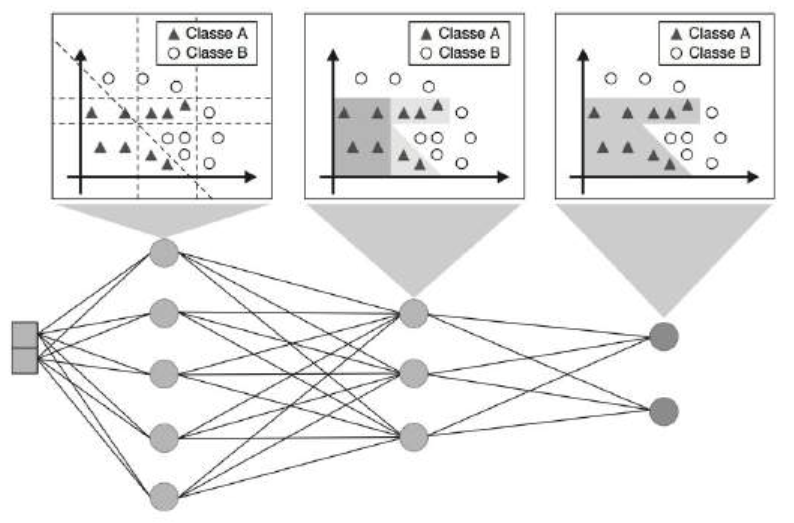
\includegraphics[width=.8\textwidth]{./img/mlp.png}
\caption{Papel desempenhado pelos neurônios em cada camada de uma RNA MLP. Fonte: \cite{Faceli:Livro}.}
\label{fig:mlp}
\end{figure}

O aprendizado das RNAs se dá por meio de um processo iterativo de ajustes aplicado a seus pesos, fazendo com que o modelo obtenha melhor desempenho, normalmente medido pela acurácia preditiva. Esses algoritmos, são formados por um conjunto de regras bem definidas que determinam quando e como dever ser alterado o valor de cada peso \cite{Faceli:Livro}. Um método popular para o aprendizado supervisionado de MLPs é o algoritmo de \emph{backpropagation}, que consiste em duas fases: uma fase pra frente (\emph{forward}) e outra pra trás (\emph{backwards}). Na fase \emph{forward}, os pesos sinápticos da rede são fixos e o sinal de entrada é propagado pela rede, camada por camada, até atingir a saída. Na segunda fase \emph{backwards}, um sinal de erro é produzido comparando a saída da rede com uma resposta desejada. O sinal de erro resultante é propagado através da rede, camada por camada, porém a propagação é realizada pra trás \cite{Faceli:Livro,Haykin:NeuralNetworksBook}. Nesta segunda fase, ajustes sucessivos são feitos nos pesos da rede utilizando o algoritmo do gradiente descendente \cite{Teresa:Livro}.

As CNNs são uma categoria de RNAs especialmente voltadas para lidar com dados de alta dimensionalidade, tais como imagens, áudio, vídeo, etc. Elas operam de maneira muito semelhante às RNAs MLP, mas com uma diferenças fundamentais no tocante aos neurônios e aos tipos de camada. Os neurônios artificiais convolucionais são caracterizados por um filtro que é convoluído com a entrada, permitindo uma extração apropriada de características frente ao tipo de dado de entrada, pois são capazes de abstrair características como texturas, contornos, cores, etc. As camadas compostas de neurônios convolucionais são chamadas de camadas convolucionais \cite{Khan:2018}.

As CNNs também fazem uso de camadas de \emph{pooling}, tipicamente dispostas após as camadas convolucionais, com vistas a promover uma redução de dimensionalidade, produzindo representações condensadas das entradas. As diversas camadas convolucionais e de \emph{pooling} na arquitetura de uma CNN são responsáveis pela extração automática de características da entrada, as quais passam por camadas densas, tipicamente dispostas ao final da CNN, com vistas a produzir a saída desejada para a tarefa em questão (classificação, regressão, etc.) \cite{Buduma:2018,Chollet:2017}.

Como a extração de características nas CNNs é automática e massiva, é importante utilizar alguma estratégia para descartar valores que podem estar associados à ruído ou que possuem pouca influência na saída do modelo. Isso é feito com camadas de \emph{Dropout}, as quais são compostas de neurônios com limiar para descartar aleatoriamente certas conexões ao longo do treino, colaborando para a regularização e para a diminuição no número de parâmetros ajustáveis das CNNs \cite{Buduma:2018,Chollet:2017}.

As CNNs são tipicamente utilizadas perante o paradigma de Aprendizado Supervisionado com especial destaque para tarefas de classificação em Visão Computacional, representando o estado da arte em diversos problemas nesse domínio \cite{Khan:2018}. Citam-se algumas arquiteturas canônicas de CNNs, tais como, LeNet, AlexNet, Inception e VGG-16, as quais obtiveram desempenho notável em diversas edições do \emph{ImageNet Large Scale Visual Recognition Challenge} (LSVRC) \cite{ILSVRC15}.


\section{Detecção de Objetos com Redes Neurais Convolucionais} \label{sec:fundamenta:deteccao}
%!TEX root=../../sbc-template.tex

A detecção e o reconhecimento de objetos são componentes chave para a maioria dos sistemas de visão computacional e determinam o desempenho de muitos aplicativos, como rastreamento, recuperação, vigilância por vídeo e legendagem de imagens. O desempenho da detecção e reconhecimento de objetos depende muito da qualidade das características extraídas e da robustez dos modelos, uma vez que a aparência das imagens pode ser influenciada por diversos fatores, como condições de iluminação, pose, refletância dos objetos e características intrínsecas das câmeras \cite{Jiang:2019}. Por isso que, nos últimos anos, as redes neurais profundas ganharam espaço nos problemas mais complexos da atualidade como processamento de imagens e visão computacional. A Figura \ref{fig:example-detection} ilustra a detecção de várias classes para uma mesma entrada.

\begin{figure}[H]
    \centering
    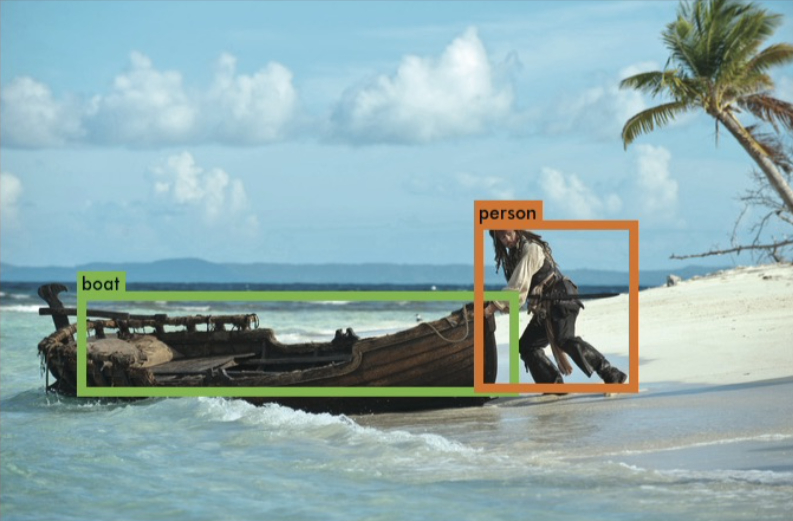
\includegraphics[width=.7\textwidth]{img/example-detection.png}
    \caption{Tarefa de detecção de objetos sendo realizada. Fonte: \cite{Yolo:2015}}
    \label{fig:example-detection}
\end{figure}

É importante salientar que a classificação de uma imagem, isto é, um modelo classificar o conteúdo de uma foto, por exemplo, é diferente de detectar exatamente em que área da foto o objeto encontra-se. Com isso, é possível perceber que os modelos que abordam essa tarefas precisam ser mais robustos pois existe agora uma nova etapa na qual o modelo precisa realizar: definir na imagem quais os limites da entidade em questão. Em resumo, o modelo, para detecção de objetos numa imagem, deve ser capaz de identificar a localização de uma ou mais entidades (as classes) além de emitir qual classe ela(s) pertence(m) \cite{Michelucci:2019}.

A métrica necessária para verificar a qualidade dessa tarefa é justamente a interseção da área correspondente ao objeto (resultado esperado) em relação à área detectada sobre a união dessas áreas em questão, conhecida também como Interseção sobre União (IoU) \cite{Chollet:2017}. O desafio está em detectar as áreas das entidades na imagem. Uma das primeiras estratégias que solucionaram esse problema é a Aproximação da Janela Deslizante: uma certa área (a janela deslizante) igual ou menor que a imagem total é inicialmente definida e percorre todas as combinações possíveis com a imagem original, calculando o IoU. Em seguida, outra janela deslizante é definida com outro tamanho e o processo é refeito. No fim, verifica-se qual IoU foi o mais satisfatório para o resultado final da detecção da entidade. Essa estratégia é bastante custosa pois podem existir milhares de combinações possíveis em cada teste, razão pela qual não é muito utilizada \cite{Michelucci:2019}.

Outra estratégia para a detecção é conhecida como Region-Based CNN (R-CNN), ou CNN Baseada em Regiões. Como a estratégia das janelas deslizantes necessita de muitas combinações, a baseada em regiões propõe inicialmente 2000 regiões na imagem. Em seguida as regiões adjacentes são unidas baseadas em características similares como cor, textura e forma, sendo possível visualizar a técnica na Figura \ref{fig:selective-search}. Então, com menos regiões para serem analisadas, o cálculo de IoU é também realizado e a melhor métrica acaba escolhendo também a melhor região para o resultado \cite{Michelucci:2019}.

\begin{figure}[H]
    \centering
    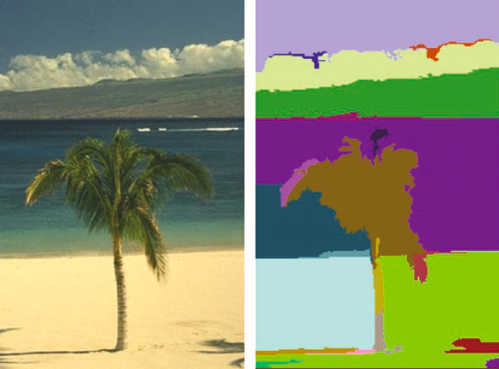
\includegraphics[width=.7\textwidth]{img/selective-search.png}
    \caption{Pesquisa seletiva destacando regiões de interesse. Fonte: \cite{Michelucci:2019}}
    \label{fig:selective-search}
\end{figure}

Como as R-CNN são modelos mais complexos devido ao janelamento, uma solução para torná-las mais rápidas foi desenvolvida: a chamada Fast R-CNN. A razão pela qual esse algoritmo é mais rápido que o R-CNN está no fato de que torna-se desnecessário alimentar 2000 propostas de região para a rede neural convolucional, o processo é realizado uma única vez com a extração de mapa de características da imagem, similar às características semelhantes das regiões inicializadas nas R-CNN \cite{Michelucci:2019}.

Mesmo as Fast R-CNN tendo se mostrado mais rápidas que as R-CNN convencionais, o custo para treinar o modelo ainda é alto visto que a pesquisa para selecionar as regiões propostas é ainda gargalo do algoritmo. Com isso, uma outra solução para essa etapa foi desenvolvida: utilizar uma outra rede neural para aprender as regiões de dados rotulados, removendo então a etapa demorada de procura seletiva das regiões. Assim, esse modelo foi chamado de Faster R-CNN por ser significativamente mais rápido que R-CNN e Fast R-CNN \cite{Michelucci:2019}.



\section{Família YOLO} \label{sec:fund:yolo}
%!TEX root=../../sbc-template.tex

Com a popularização das R-CNNs e o crescente interesse prático nas tarefas de detecção de objetos, em 2016 foi proposta a R-CNN YOLO (acrônimo para \emph{You Only Look Once}), a qual se propõe a realizar as tarefas de localização e classificação de múltiplos objetos em uma única etapa (\emph{single-shot}) \cite{Redmon:YOLOoriginal}. Essa R-CNN mostrou-se significativamente mais rápida para detecção do que os modelos anteriores do mesmo tipo disponíveis na literatura \cite{Michelucci:2019}.

Conforme ilustrado na Fig. \ref{fig:yolo_grid}, a abordagem de detecção de objetos por R-CNNs YOLO consiste nos seguintes passos: primeiramente há a divisão da imagem de entrada em uma grade de dimensões $S \times S$; em seguida, para cada célula, há uma verificação se há um objeto cujo centro é englobado pela mesma; para as células em que tal verificação foi afirmativa, calcula-se a quantidade $B$ de caixas delimitadores com seus respectivos coeficientes de confiança -- obtidos por meio da multiplicação da métrica IoU (do inglês, \emph{Intersection Over Union}) com a probabilidade da célula conter um certo objeto de uma dada classe -- refletindo numericamente o quão acurada está uma caixa delimitadora que contém o objeto; por fim, células adjacentes com alta confiança para um mesmo tipo de objeto são unificadas, culminando na previsão das coordenadas das caixas e seus respectivos rótulos \cite{Michelucci:2019}.

\begin{figure}[H]
    \centering
    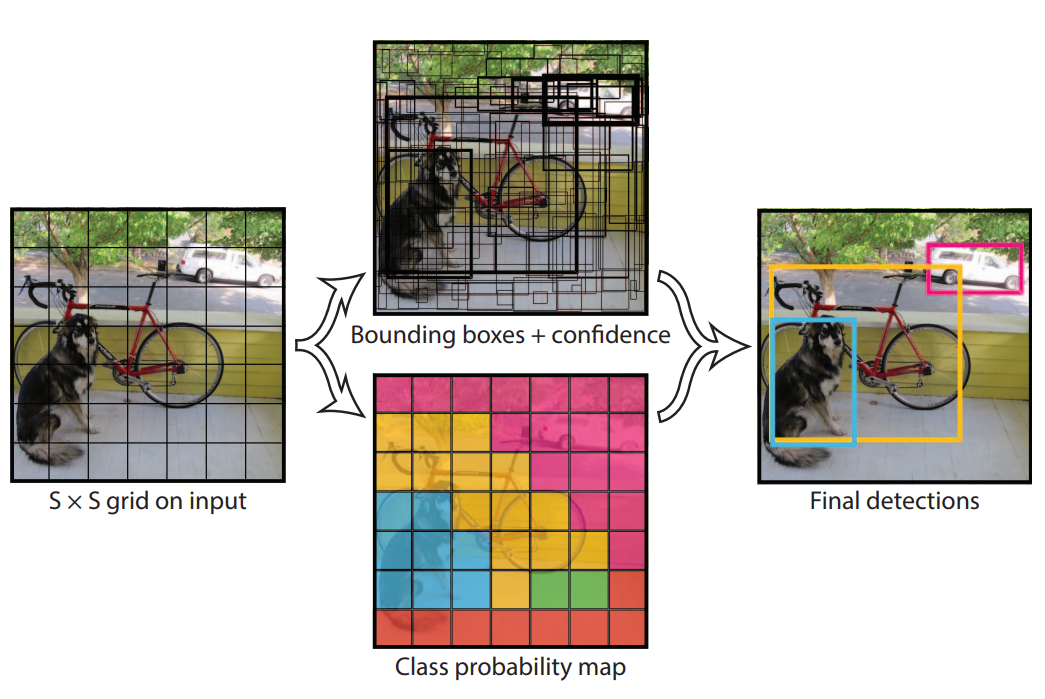
\includegraphics[width=0.70\textwidth]{img/yolo-approach}
    \caption{Abordagem da YOLO para detecção de objetos.
    Fonte: \cite{Redmon:YOLOoriginal}.}
    \label{fig:yolo_grid}
\end{figure}

A arquitetura utilizada na YOLOv1 (primeira versão) foi inspirada na CNN Inception pré-treinada com pesos oriundos da base de dados ImageNet \cite{ImageNet}. Esta arquitetura é constituída por $20$ camadas convolucionais seguidas por $2$ camadas totalmente conectadas. Ao invés de usar os módulos Inception originais, os autores da YOLO optaram por utilizar camadas de \emph{pooling} com filtros de dimensões $1\times 1$ para redução de dimensionalidade seguidos de camadas convolucionais com filtros $3 \times 3$, conforme ilustrado na Figura \ref{fig:yolo_arch}.

\begin{figure}[H]
    \centering
    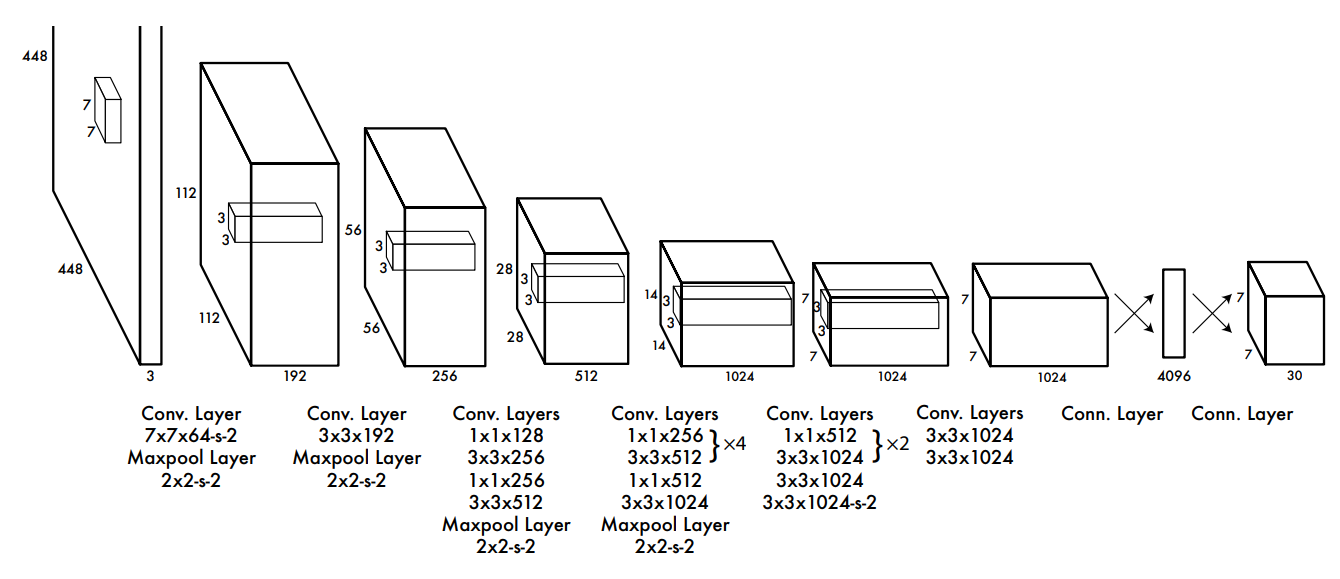
\includegraphics[width=\textwidth]{img/yolo-arquitetura}
    \caption{Arquitetura da CNN utilizada na primeira versão da YOLO.\\ Fonte: \cite{Redmon:YOLOoriginal}.}
    \label{fig:yolo_arch}
\end{figure}

% Seguir para Yolov4,  v5, v6 e v7.

Ao longos dos anos, novas técnicas e melhorias foram incorporadas em versões atualizadas de modelos da Família YOLO. Para a YOLOv4, por exemplo, utilizou-se o \emph{backbone} CSPDarkNet53, tornando-a duas vezes mais rápida que outras arquiteturas de referência na época do seu lançamento. Ainda, comparando com a sua versão anterior (YOLOv3) as métrica AP e FPS foram melhoradas em $\SI{10}{\percent}$ e $\SI{12}{\percent}$, respectivamente \cite{Bochkovski:YOLOv4}.

A YOLOv5 decorreu logo após a proposição da YOLOv4 tendo como maior diferença a implementação do \emph{framework} DarkNet de forma nativa com o Pytorch, o que facilitou drasticamente o treinamento e o \emph{deployment} desse modelo. A principal inovação da YOLOv5 em relação às suas antecessoras foi a introdução do \emph{Mosaic Augmentation}, uma técnica de regularização por meio do aumento artificial de dados que combina quatro imagens em quatro blocos de proporção aleatória. Conforme argumentam seus proponentes, a principal vantagem dessa inovação é a melhoria de desempenho na detecção de objetos pequenos. No sétimo \emph{release}, diferentes versões da YOLOv5 foram propostas para atender domínios específicos, citadas a seguir por ordem crescente de parâmetros e robustez: \emph{Nano}, \emph{Small}, \emph{Medium}, \emph{Large} e \emph{XLarge}. Os modelos mais simples visam aplicações embarcadas por serem mais leves, enquanto os mais complexos foram projetados para problemas mais difíceis, com imagens de maior dimensão, grande número de classes e tamanho de caixas delimitadoras bastante variados \cite{Jocher:YOLOv5}. A Figura \ref{fig:yolov5} ilustra o desempenho das diferentes versões da YOLOv5 perante a base de dados MS COCO \cite{Microsoft:COCO}, um \emph{benchmark} da literatura para detecção de objetos.

\begin{figure}[h!]
    \centering
    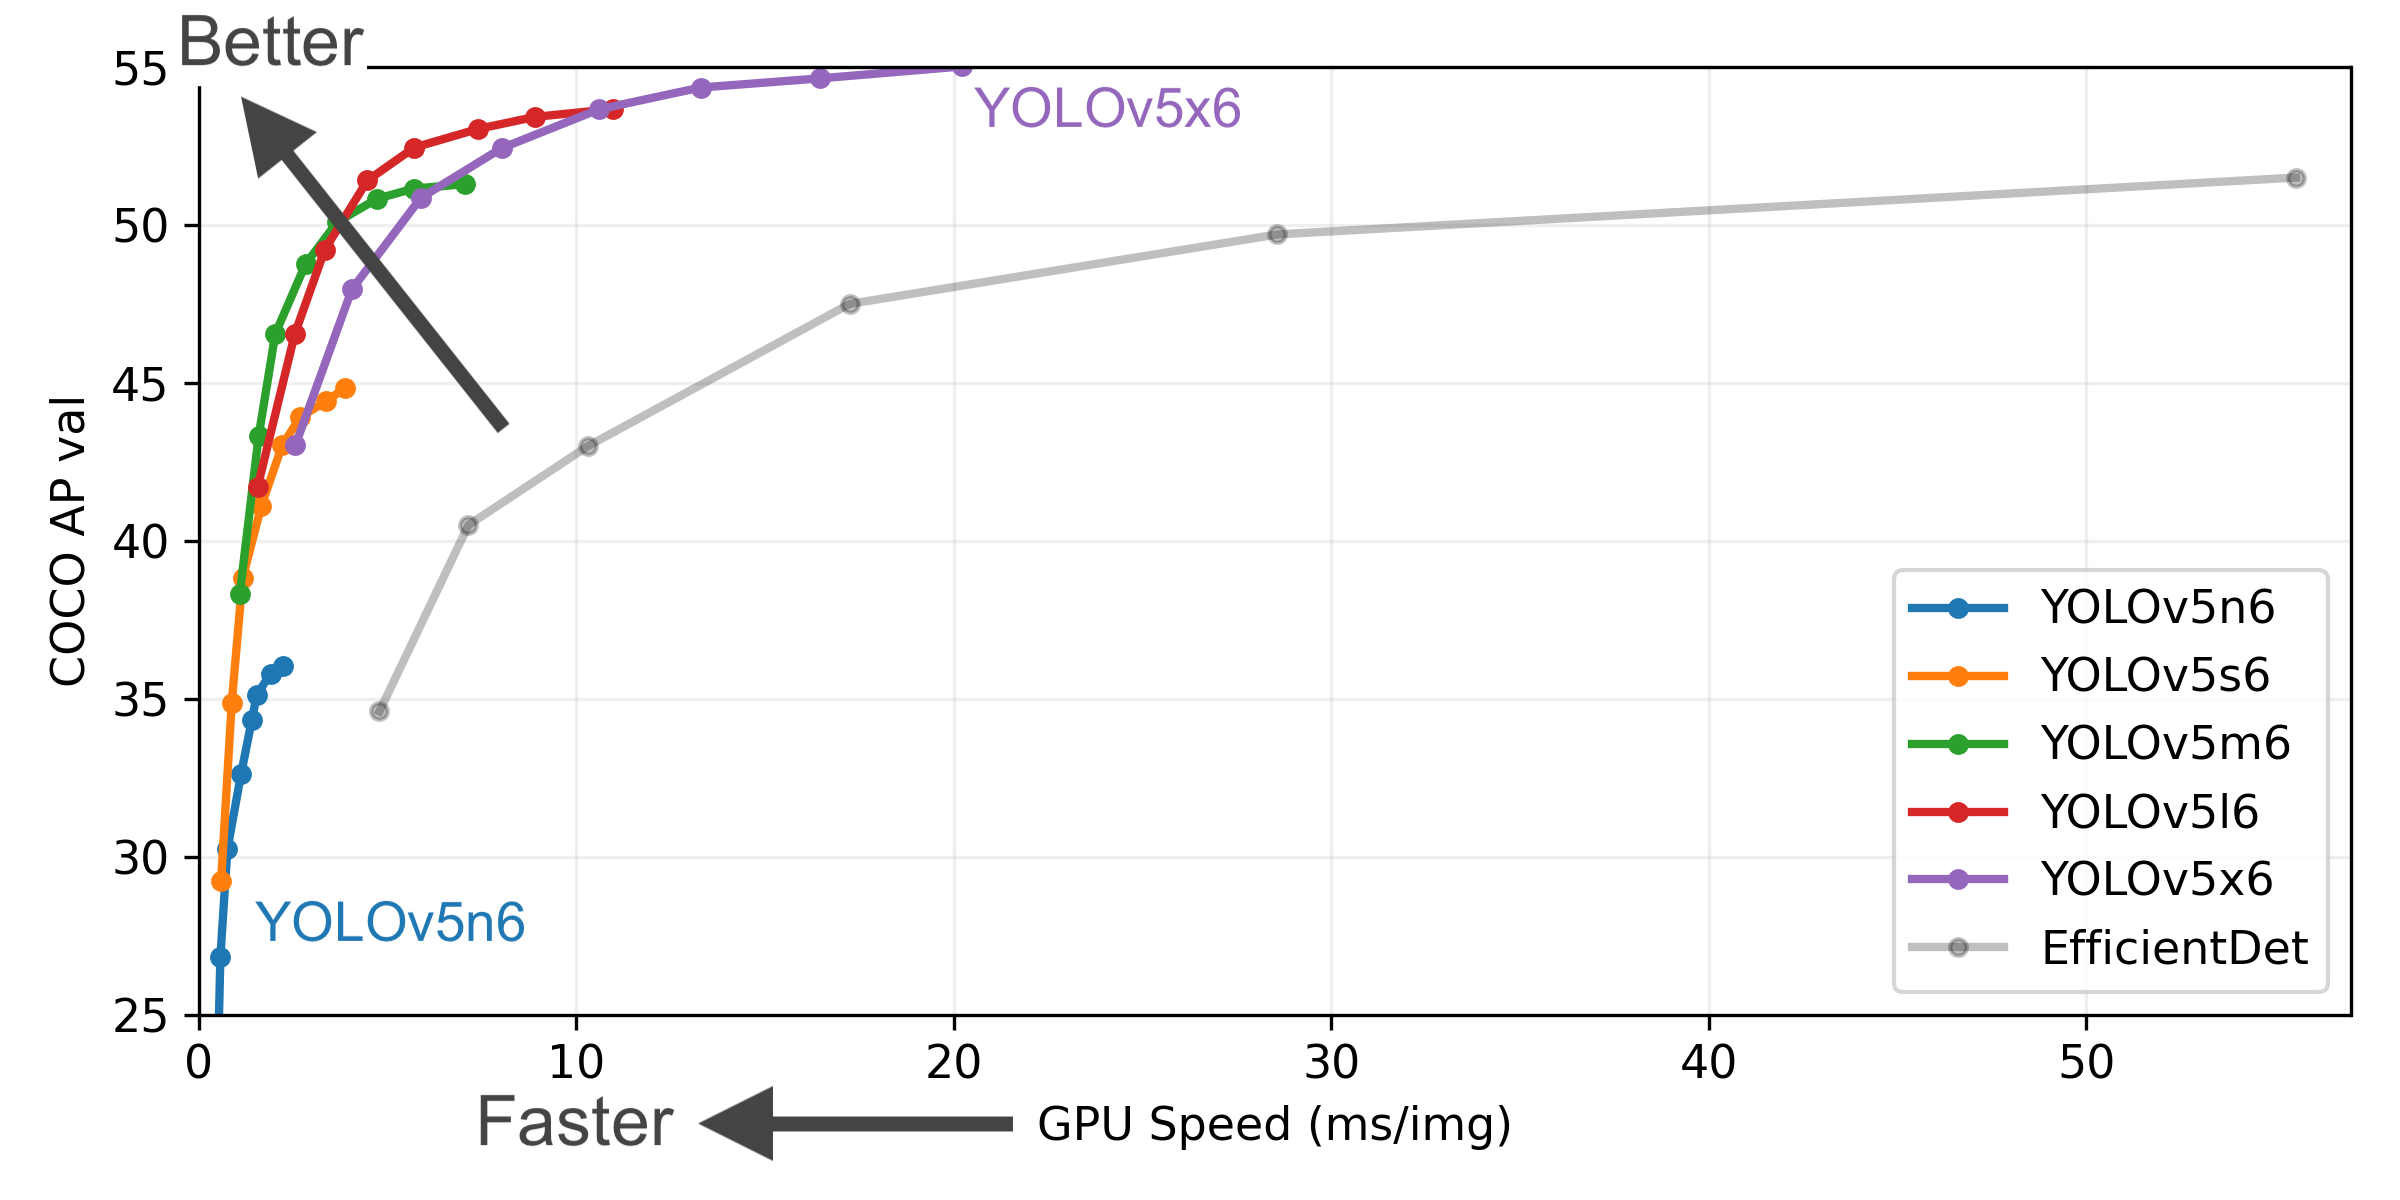
\includegraphics[width=0.8\textwidth]{./img/yolov5}
    \caption{Desempenho dos modelos YOLOv5 perante o MS COCO.\\ Fonte: \cite{Jocher:YOLOv5}.}
    \label{fig:yolov5}
\end{figure}

Outras versões da YOLO foram propostas por diferentes autores, mas nem todas se consolidaram perante a comunidade técnico-científica pois, apesar de apresentarem um bom desempenho no \emph{benchmark} MS COCO, não reproduziam tal eficiência em problemas de outros domínios. Ademais, era notável a dificuldade no treinamento em face da carência de documentação e de uma comunidade pequena de usuários. Como exemplo, cita-se o caso da YOLOv6 \cite{YOLOv6}.


A YOLOv7 deu continuidade ao aprimoramento dos modelos da Família YOLO ao incorporar um processo denominado reparametrização, com o intuito de diminuir o tamanho do modelo para \emph{deployment}, o que é especialmente útil para sistemas embarcados. Também faz uso de \emph{Feature Pyramid Networks} em sua arquitetura, as quais empilham camadas convolucionais e produzem previsões em diferentes escalas, colaborando para um melhor desempenho. Diferentemente das versões anteriores, propôs uma arquitetura padrão e uma estratégia de dimensionamento em escala para outras quantidades de parâmetros, sejam elas maiores ou menores \cite{yolov7}. A Figura \ref{fig:yolo-arch} apresenta uma análise comparativa entre os diferentes modelos da Família YOLO recém propostos na literatura perante o MS COCO.


\begin{figure}[h!]
    \centering
    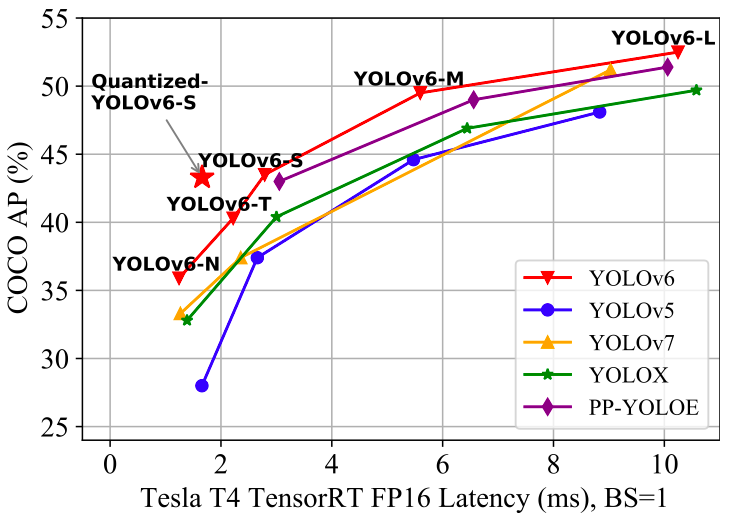
\includegraphics[width=0.75\textwidth]{img/yolo-latest-version}
    \caption{Comparação entre as últimas versões da YOLO propostas na literatura. O eixo vertical denota a eficiência do modelo e o eixo horizontal denota o tempo de treinamento.\\ Fonte: \cite{YOLOv6}.}
    \label{fig:yolo-arch}
\end{figure}

\section{Trabalhos Relacionados} \label{sec:fund:relacionados}
\iffalse \begin{frame}{Trabalhos relacionados}
    \begin{itemize}
        \item Primeiros trabalhos: uso de sensores, tais como acelerômetro e giroscópio, para reconhecer danos por meio da amplitude da vibração detectada \cite{caodl}
        \ \ \newline
        \item \alert{\emph{Global Road Damage Detection Challenge}} (GRDDC):
        \begin{itemize}
            \item \alert{RDD2020}: \emph{Road Damage Detection and Classification dataset} \cite{RDD2020:Dataset2}
            \item Equipes realizaram a etapa de testes em duas bases de dados privadas
            \item $\SI{67}{\percent}$ das melhores soluções utilizaram modelos de família YOLO e as 3 melhores soluções utilizaram comitês de R-CNNs \cite{arya2020global}
            \item \alert{Melhor solução}: $F_1\textrm{-\emph{Score}} \approx 0,67$, YOLOv5, Test Time Augmentation, $3,08$ FPS \cite{Hegde2020:Campeao}
        \end{itemize}
    \end{itemize}
\end{frame}
\fi